\chapter{Fundamentals and Related Work}
\label{chap:fundamentals}
The first three sections of this chapter are the fundamental concepts that are required to understand the intention oriented organizational modeling approach to be discussed in the Section \ref{sec:topdownapproach} of Chapter \ref{chap:approach}. The fourth section provides a brief introduction about Informal Process Essentials (IPE) approach. The fifth section discusses the conceptual model of the intention-oriented organizational modeling. The final section discusses the Executing Informal Processes (InProXec) method which helps to realize the IPE approach in organizations.

%%%%%%%%%%%%%%%%%%%%%%%%%%%%%%%%%%%%%%%%%%%%%%%%%%%%%%%%%%%%%%%%%%%%%%%%%
\section{Definitions of the Terms}
\label{sec:termdefinitions}
%%%%%%%%%%%%%%%%%%%%%%%%%%%%%%%%%%%%%%%%%%%%%%%%%%%%%%%%%%%%%%%%%%%%%%%%%
In this section, the definitions of terminologies that are used throughout this document are provided briefly.

\textit{Business Process} -  A business process has been defined as set of activities whose final output is accomplishment of a goal \cite{Weske2012}.  

\textit{Business Logic} - Business logic refers to the activities that need to be done to execute the corresponding business process \cite{Weske2012}. 

\textit{Business Process Model} - Business process model is a model to capture recurring activities during business process execution and enact them in an automated fashion for re-using the stored knowledge \cite{Weske2012}. 

\textit{Informal Process Essentials} - Informal Process Essentials (IPE) is a resource-driven approach that enables describing process declaratively, i.e., without describing how the intention is achieved and providing only information about what has to be achieved \cite{Sungur2014a}. 

\textit{OASIS Topology and Orchestration Specification for Cloud Applications} (TOSCA) - TOSCA is an OASIS (Organization for the Advancement of Structured Information Standards) standard to describe composite applications and their management \cite{Kopp2013}.  

\textit{Winery} - Winery is a modeling tool offering a web-based environment for graph-based modeling of application topologies and defining reusable components and their relationship types. It is an editor to create TOSCA documents \cite{Kopp2013}. 

%%%%%%%%%%%%%%%%%%%%%%%%%%%%%%%%%%%%%%%%%%%%%%%%%%%%%%%%%%%%%%%%%%%%%%%%%
\section{Human-centric Process}
\label{sec:humancentric}
%%%%%%%%%%%%%%%%%%%%%%%%%%%%%%%%%%%%%%%%%%%%%%%%%%%%%%%%%%%%%%%%%%%%%%%%%
The role of humans in organizations has been evolving over time. The shift from "personnel" to "human resources" acknowledges the importance of humans as organizational resources. Today's organizations are dynamic in nature due to frequent changes that happen inside the organizations. For example, organizational changes like addition of new organizational alliances, new structures and hierarchies, new ways of assigning work and a very high rate of changes like changes in the workforce, including employees' priorities, capabilities and demographic characteristics. Thus, it is impossible to do one hundred percent perfect forecasting of dynamically changing processes in an organization.

In order to manage such a dynamic environment, organizations need skilled human resources with the previous knowledge of handling the unforeseen scenarios. Thus, human resources are vital part of any organization as they have skills of acute future orientation to understand the changing organizational environment. Humans in organizations carry out many important activities. \textit{Managers} and \textit{Human Resource} (HR) professionals organize jobs of each and every human in the organization so that they can effectively perform these jobs. Thus, humans in any organization are viewed as resources of the organization which is a contemporary part of \textit{Human Resource Management} \cite{Bianca2016}.

Collaborations exist in every level of an organization. For example, at management levels of an organization, managers and HR professionals work together to assign employees their roles and task in the organization. This helps the employees of the organization in adapting to its environment. In a flexible organization, employees' roles and responsibilities changes dynamically based on the requirements and business priorities. Thus, the need for network of representations between the human resources, that helps to identify human resources based on their roles is arising. This network of representation sets up an environment to support the collaborative work of business related process. This kind of support to represent human resource network has been realized in the work by author Canko \cite{Canko2015}. The concept of \textit{virtual human representation} described by the author is an extension of actor-concept described in the \textit{Informal Process Essentials} \cite{Sungur2014a}. The prototype \textit{Human Resource Representation} developed in the work by author Canko, saves the information such as capabilities, roles, responsibilities, etc., as a virtual human web ontology instance which can be reused in the  web-based environments. These kind of human representations are highly helpful to organizations with dynamically changing resources. These representations can describe and match resources with their capabilities based on the requirements \cite{Canko2015}.

%%%%%%%%%%%%%%%%%%%%%%%%%%%%%%%%%%%%%%%%%%%%%%%%%%%%%%%%%%%%%%%%%%%%%%%%%
\section{Organizational Modeling Notations}
\label{sec:resourcecentricorganizationalmodeling}
%%%%%%%%%%%%%%%%%%%%%%%%%%%%%%%%%%%%%%%%%%%%%%%%%%%%%%%%%%%%%%%%%%%%%%%%%
The organizational modeling element notation has been selected based on the guidelines mentioned in the literature \cite{Moody2009} and these notations are adopted from another thesis work \cite{Sierr2015}. Though these notations modeling are not part of this master thesis, this is provided in this section for the sole purpose of aiding the reader to understand the concepts better through graphical representations. Also, by observing  the fact that business process modelers are already well-known with the present process modeling notations such as Business Process Modeling Notation 2.0 (BPMN) \cite{bpm2011} and ArchiMate notation \cite{arc2013}, the shape depiction of organizational model elements has been designed similar to those existing process notations. 

Due to the importance of shapes in expressing information visually, the notations are chosen in such a way that each element of organizational notations differ by shape. A legend holding respective name of each notation is shown in the following images to denote the meaning of each shape. The description of each element in the organizational model notation is shown in the Table \ref{tab:notations}. 

\begin{center}
	\begin{longtable}{p{3cm}p{10cm}p{3cm}}
		\toprule 
		\textbf{Element} & \textbf{Definition} & \textbf{Notation} \\
		\midrule
		\endfirsthead
		Intention 			& Intention is a desired objective or state that must be reached by organizations or individuals to achieve an expected outcome \cite{DelaVaraGonzalez2007}. & \begin{center} 
\includegraphics[width= 0.07\textwidth]{Intention.pdf}  \end{center}  \\
		
		Capability	&  Capability is an ability that should be possessed by a resource that work towards the achievement of one or several intentions \cite{Sierr2015}.   & \begin{center} 
\includegraphics[width= 0.07\textwidth]{Capability.pdf} \end{center}  \\
		
		Context				& The environment that forms the setting for an event, statement, or idea and in terms of which it can be fully understood. There are two contexts: initial and final. Initial context is the situation which describes the driving force that trigger the informal process to start. Final context is the expected situation once the informal process has finished. Both initial and final context are represented by an hexagonal shape except the final context has thick edges than the initial context \cite{Sierr2015}.  & \begin{center} 
\includegraphics[width= 0.07\textwidth]{Context.pdf} \end{center}   \\
		\newline
		Strategy		& \newline  A strategy is an approach, a manner or a means to achieve an intention \cite{Bider2005}.   & \begin{center} 
\includegraphics[width= 0.07\textwidth]{Strategy.pdf} \end{center}  \\
		
		Resource					& The people or tools that work towards the achievement of an intention. & \begin{center} 
\includegraphics[width= 0.07\textwidth]{Resource.pdf} \end{center}  \\
		
		Relationship				& Relationship between two elements is used to specify how the source and target element is related.  & \begin{center} 
\includegraphics[width= 0.07\textwidth]{Relationship.pdf} \end{center}   \\
		
		\bottomrule
		\caption{Organizational Modeling Notations}
		\label{tab:notations}		
	\end{longtable}	
\end{center}

%%%%%%%%%%%%%%%%%%%%%%%%%%%%%%%%%%%%%%%%%%%%%%%%%%%%%%%%%%%%%%%%%%%%%%%%%
\section{Overview of the Informal Process Essentials}
\label{sec:basicconcepts}
%%%%%%%%%%%%%%%%%%%%%%%%%%%%%%%%%%%%%%%%%%%%%%%%%%%%%%%%%%%%%%%%%%%%%%%%%
In this section, we provide an overview about the concepts introduced in the approach Informal Process Essentials (IPE) \cite{Sungur2014a}. As mentioned earlier, the modeling elements of the proposed approach in the following Chapter \ref{chap:approach} are adapted from IPE approach. Hence, IPE approach serves as an important related work required to understand the proposed approach. 

The authors describe following as the properties of an informal process (1) business logic of an informal process is not defined explicitly before the enactment, (2) an informal process is collaborative in nature which requires resources with interrelationships, (3) a resource can participate in multiple informal processes and (4) resources associated with an informal process can change dynamically.

The authors also provide the following requirements that support informal processes with the above described properties. The summarized requirements are (1) ability to represent informal process as models and ability to execute it, (2) due to involvement of multiple resources, ability to define relationships among the resources, (3) resources should be visible in the process representations and (4) support for dynamically changing resources. 

The authors also compare existing approaches in the literature with the above requirements. It has also been concluded that analyzed approaches only satisfy some of the requirements but not all the requirements completely. Thus, the authors propose the IPE approach that satisfies all the requirements. In this IPE approach, resources are related to each other and work towards achievement of an intention, i.e., a goal.   

As mentioned in Section \ref{sec:termdefinitions}, resources are drivers to achieve intentions in the informal processes. Sungur et al. \cite{Sungur2014a} state that when the desired process result is repeated, then the same set of resources can be selected and engaged towards collective intention of that process. IPE models begin from an initial context and after achieving the main intention it results in another context. The relationship between IPE approach and the conceptual model of intention-oriented organizational modeling is explained in the next section.

%%%%%%%%%%%%%%%%%%%%%%%%%%%%%%%%%%%%%%%%%%%%%%%%%%%%%%%%%%%%%%%%%%%%%%%%%
\section{Intention-oriented Organizational Modeling - Conceptual Model}
\label{sec:entitytypesrepresentation}
%%%%%%%%%%%%%%%%%%%%%%%%%%%%%%%%%%%%%%%%%%%%%%%%%%%%%%%%%%%%%%%%%%%%%%%%%
The conceptual model of organizational modeling elements used in intention-oriented organizational modeling is shown in the Figure \ref{fig:entitymodel}. This conceptual model shows that intention contains multiple strategies. An intention can be achieved through a strategy, which is a plan of action designed to meet the intention. The strategies require capabilities and contain IPE processes. The IPE processes realize strategies. The capabilities can be further resolved into resources. Thus, starting from defining intentions, we define strategies then required capabilities and IPE models. The capabilities and process models define the required resources. 

Organizational process modeling of this approach is an \textit{intention-oriented} as they support modeling based on intention and required resources thrive to successfully achieve organizational intention by using qualified autonomous agents, i.e., actors under certain \textit{context definitions}. Emerging intentions can result in the requirement of new capabilities, i.e., an ability required to achieve an intention.

\begin{figure}
	\centering
	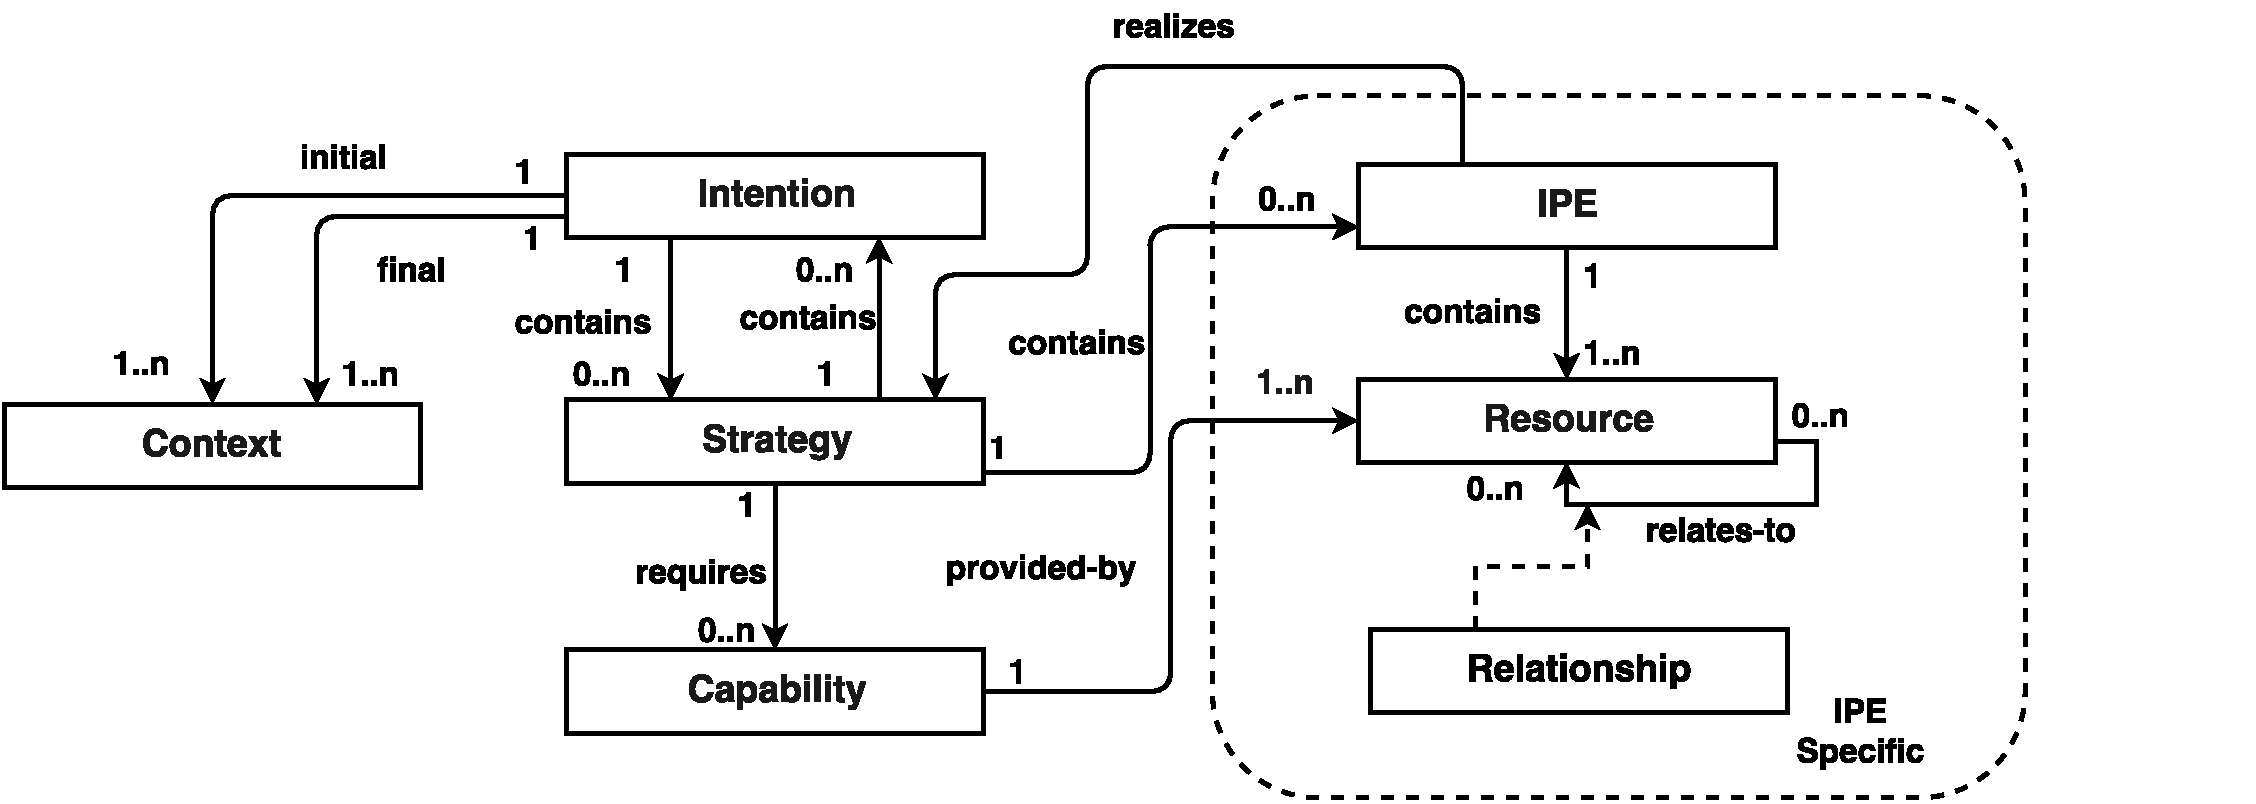
\includegraphics[width= 1.1\textwidth]{entity.pdf}
	\caption{Intention-oriented Organizational Modeling - Conceptual Model}
	\label{fig:entitymodel}
\end{figure}

 An informal process targets for accomplishment of an intention. The intention can be refined by defining strategies, which can then be further refined recursively as independent informal processes. The intention-based approach enables describing processes declaratively, i.e., without describing \textit{how} the intention is achieved, and providing only information about \textit{what} is achieved. The IPE approach suggests that this avoids need for predefined business logic in the representations of informal processes. Each resource can be related to another resource in the context of an informal process using predefined or custom \textit{relationships}. Since IPE realizes strategy, each informal process starts from a context, i.e., \textit{initial context} and aims to achieve an intention. After accomplishing the intention, there is a resulting context called as \textit{final context}. The beginning state before achieving an intention is called as initial context and the end state after achieving an intention is called as final context.

%%%%%%%%%%%%%%%%%%%%%%%%%%%%%%%%%%%%%%%%%%%%%%%%%%%%%%%%%%%%%%%%%%%%%%%%%
\section{Executing Informal Processes}
\label{sec:inproxec}
%%%%%%%%%%%%%%%%%%%%%%%%%%%%%%%%%%%%%%%%%%%%%%%%%%%%%%%%%%%%%%%%%%%%%%%%%
In this section, we present an overview about the \textit{Executing Informal Processes} (InProXec) method \cite{Sungur2015}. Implementing IPE approach in organization requires the application of InProXec with different phases. The InProXec method enables modeling of informal processes and automated provisioning of resources modeled in these processes. Since this thesis work, is realizing intention-oriented modeling of organizations, it covers second phase of InProXec which is "\textit{Model Informal Process}" (P2). The method described in Figure \ref{fig:inprocxec_steps}, initializes informal process models in an automated fashion. In the following paragraphs, a short overview about different phases of the InProXec method has been provided and with a detailed description about the second phase of the \textit{InProXec} method is provided in the Section \ref{sec:informalprocessmodeling} of Chapter \ref{chap:approach}. As shown in the Figure \ref{fig:inprocxec_steps}, the InProcXec method consists of three different phases:

\begin{figure}
	\centering
	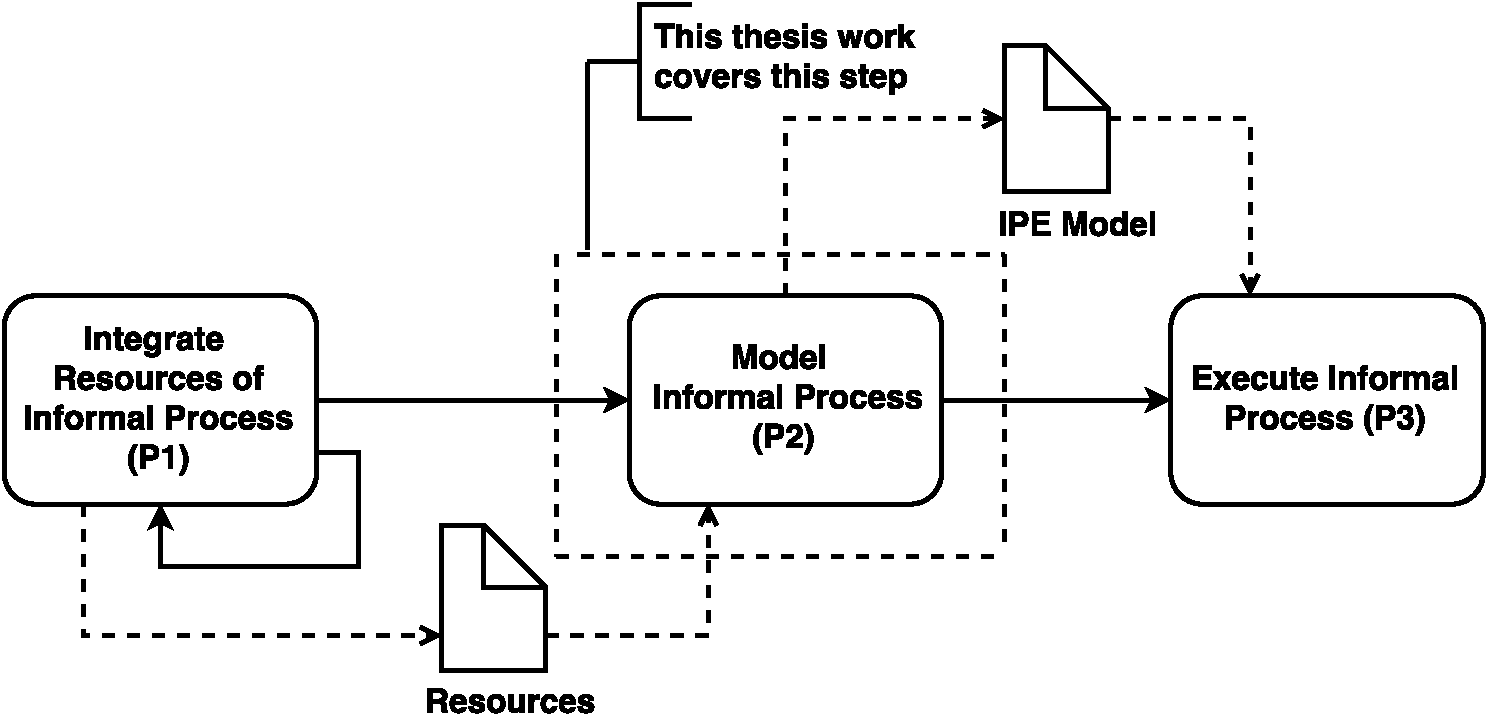
\includegraphics[width= 0.8\textwidth]{InProXec_Steps.pdf}
	\caption{Steps of the InProXec approach}
	\label{fig:inprocxec_steps}
\end{figure} 



\textit{Integrate Resources of Informal Processes (P1)} - The first phase aims for creating the required infrastructure to enable modeling and automated initialization of informal processes. This is because the required modeling tools of the informal processes modeling has to be presented to the business experts, as they require it for next phase P2. Thus, the required resources for informal process modeling are allocated through services developed by technical experts during this phase. The final output of this phase, \textit{integrated resources} are used by phase P2. 

\textit{Model Informal Processes (P2)} - This phase makes use of resources made available in the first phase P1. Based on these resources, business experts can create informal process models. As a contribution of this thesis, phase P2 has been explained in detail in the following Section \ref{sec:informalprocessmodeling} of Chapter \ref{chap:approach}

\textit{Execute Informal Processes (P3)} - Initialization of models developed in phase P2 happens automatically using the services developed in phase P1. When an IPE Model is initialized with resources, it results in a successful initialization. This successful initialization results in an IPE Model Instance. A model instance contains additional meta-data about executed processes such as the information about start time, history of the resource model, time of changes made, etc. During this phase, the autonomous actors work towards intentions of informal processes using acquired resources and other involved resources.  











